\chapter{Method}
\label{chap:method}

To predict root-relative 3D pose solely using 2D poses, a hybrid network using \ac{vae} and \ac{gan} as discussed in \ref{subsec:vaeganhybrid} is employed. In contrast to the \ac{vae}-\ac{gan} hybrid proposed by \cite{autoencoding_beyond_pixels}, the \ac{gan} loss gradient is propogated to both the decoder and the encoder. In other words, the \ac{vae} as a whole is considered as the generator network. The overall architecture is illustrated in the Fig \ref{fig:method_arch}. This chapter entails the details and the motivations behind the design choices of the neural network such as the architecture, loss function, optimizers along with the training and evaluation procedures.

\section{Encoder}
Adding to the explanation of \ac{vae} in \ref{subsec:vae}, the role of the encoder $Q$, is to take a 2D pose $\textbf{x}_i = (x_i, y_i)$ with its root located at the joint and of upper body length of $c$ units as an input. Where $i = 1 ... J$ and $J$ denote the number of joints of the pose. And output its embedding in a $d$ dimensional latent space in the form of mean $\mu$ and standard deviation $\sigma$ of each dimension.

\begin{equation} \label{eqn:Q_fn}
    \begin{gathered}[b]
        Q_{\theta_q}(\textbf{x}) = \mu, \sigma
    \end{gathered}
\end{equation}

Where $\theta_q$ denotes the learned parameters of the encoder during training. This encoder is composed of an upsampling layer that scales the $2\!\cdot\!J$ dimensional input to match the number of hidden neurons $h$ of the encoding module. The encoding module $q$ is made of $n$ residual block composed of 2 \ac{fc} layers following the related works, to allow comparison. The encoding block is followed by 2 \ac{fc} (linear) layers that downsample the hidden representation of dimension $h$ to match the latent space dimension $d$. The output of the two downsampling layers represents the mean and standard deviation respectively. However in practice, the encoder is designed to predict log-variance instead of the standard deviation to have a better distribution of values and gradient. The layers of the encoder, decoder and the discriminator models are kept similar for simplicity and as done by the related works. The residual blocks used in all the 3 models are identical and is illustrated in the Fig \ref{fig:residual_block}.

\begin{figure}[h] \label{fig:residual_block}
    \centering
    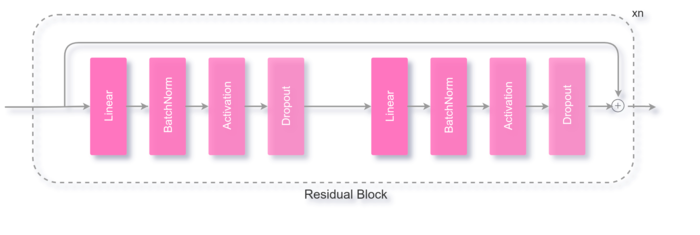
\includegraphics[width=0.45\textwidth]{figures/arch/res_block.png}
    \caption{Illustration of the residual block made of 2 Linear layers of the same input and output dimensionality. These blocks are repeated $n$ times based on the configuration of the model.
    }
\end{figure}

\section{Decoder}

The decoder $P$ takes the 2D pose embedding $z$ derived from the mean and log-variance predicted by the encoder and estimates the corresponding 3D pose $\textbf{X}_i = (x^\prime_i, y^\prime_i, z^\prime_i)$. Similar to rhe encoder, $i = 1 ... J$ and $J$ denote the number of joints of the pose. The reparametrization trick is used to make the process differentiable and induce variance. This is done by scaling the standard deviation obtained from the log-variance with a random sample $\epsilon$ from a unit gaussian distribution $\mathcal{N}(0,1)$. The sum of the scaled standard deviation and the mean gives the sample $z$.

\begin{equation} \label{eqn:P_fn}
    \begin{gathered}[b]
        z = \mu + \sigma \odot \epsilon \\
        P_{\theta_p}(z) = \textbf{X}
    \end{gathered}
\end{equation}

Where $\theta_p$ represents the learned parameters of the decoding network. Similar to the encoder, the decoder consists of an upsampling layer that scales the sample $z$ of dimensionality $d$ to match the number of hidden neurons $d$ in the decoding module. The decoding module is identical to the encoding module and consists of $n$ residual blocks composed of 2 \ac{fc} layers. This decoding module is followed by a \ac{fc} layer to downsample the neurons to predict 3D pose of dimensions $3\!\cdot\!J$. As the goal is to predict root relative pose with root at origin, the output joints are considered to be relative to the origin (0, 0, 0).

Since the predicted 3D pose is to be projected to back to 2D pose to form the reconstruction loss, the distance between the head and the pelvis joint should approximately be of unit length as explained in \ref{sec:processing}. To achieve this, a Tanh activation function is used to obtain the predicted 3D pose (all joints) in the range [-1, 1]. %TODO

\section{Reprojection}
Refering to the camera modeling section \ref{sec:camera_projection}, the 3D that corresponds to the pre-processed 2D pose is located at a fixed distance $c$ from the camera. The 3D pose is considered to be predicted relative to the origin for simplicity and symetry and is to be translated $c$ units aways from the camera. Another required adjustment is the scale. The range of coordinates predicted is in the range [-1,1]. But the length of the lower half of the pose can be longer that the upper half and usually is the case. Hence the predicted 3D pose is scaled by a factor of 1.3, which is the ratio of the mean length of the upper and lower halves. This is to enforce that the length of the upper half is ~1 unit, while covering the true range of the lower half and get the best 2D re-projection.

This scaled 3D pose prediction is directly projected from the same point of view to get a 2D projection that corresponds to the input 2D pose. This similarity is used as the reconstruction loss for a contrained optimization of the \ac{vae}.

\begin{equation} \label{eqn:proj_direct}
    \begin{gathered}[b]
        \textbf{X}^\prime = \textbf{X}*1.3 + (0,0,c) \\
        \textbf{y} = PP(\textbf{X}^\prime)
    \end{gathered}
\end{equation}

Where PP refers to perspective projection and \textbf{y} denotes the 2D projection that correspond to the input 2D pose. The scaled 3D pose is also randomly rotated by uniformly sampling an azimuth angle from the range [$-\pi, \pi$] and elevation range in the range [$-\pi/9, \pi/9$]. The 2D pose obtained from the projection of this rotated 3D pose gives a different point of view, a \textbf{\textit{novel view}} of the 3D pose that is different from the views of the subject in the dataset. This novel view is used for unconstrained optimization of the \ac{vae} using the discriminator. The elevation angle has been followed by other works but is not observed to have any visible impact.

\begin{equation} \label{eqn:proj_rotated}
    \begin{gathered}[b]
        \textbf{X}^\prime_{rot} = \textbf{R} * (\textbf{X}*1.3) + (0,0,c) \\
        \tilde{\textbf{y}} = PP(\textbf{X}^\prime_{rot})
    \end{gathered}
\end{equation}

Where \textbf{R} referes to the rotation matrix formed using the randomly sampled angles. $\tilde{\textbf{y}}$ referes to novel view of the 3D pose.

\begin{figure}[h] \label{fig:method_arch}
    \centering
    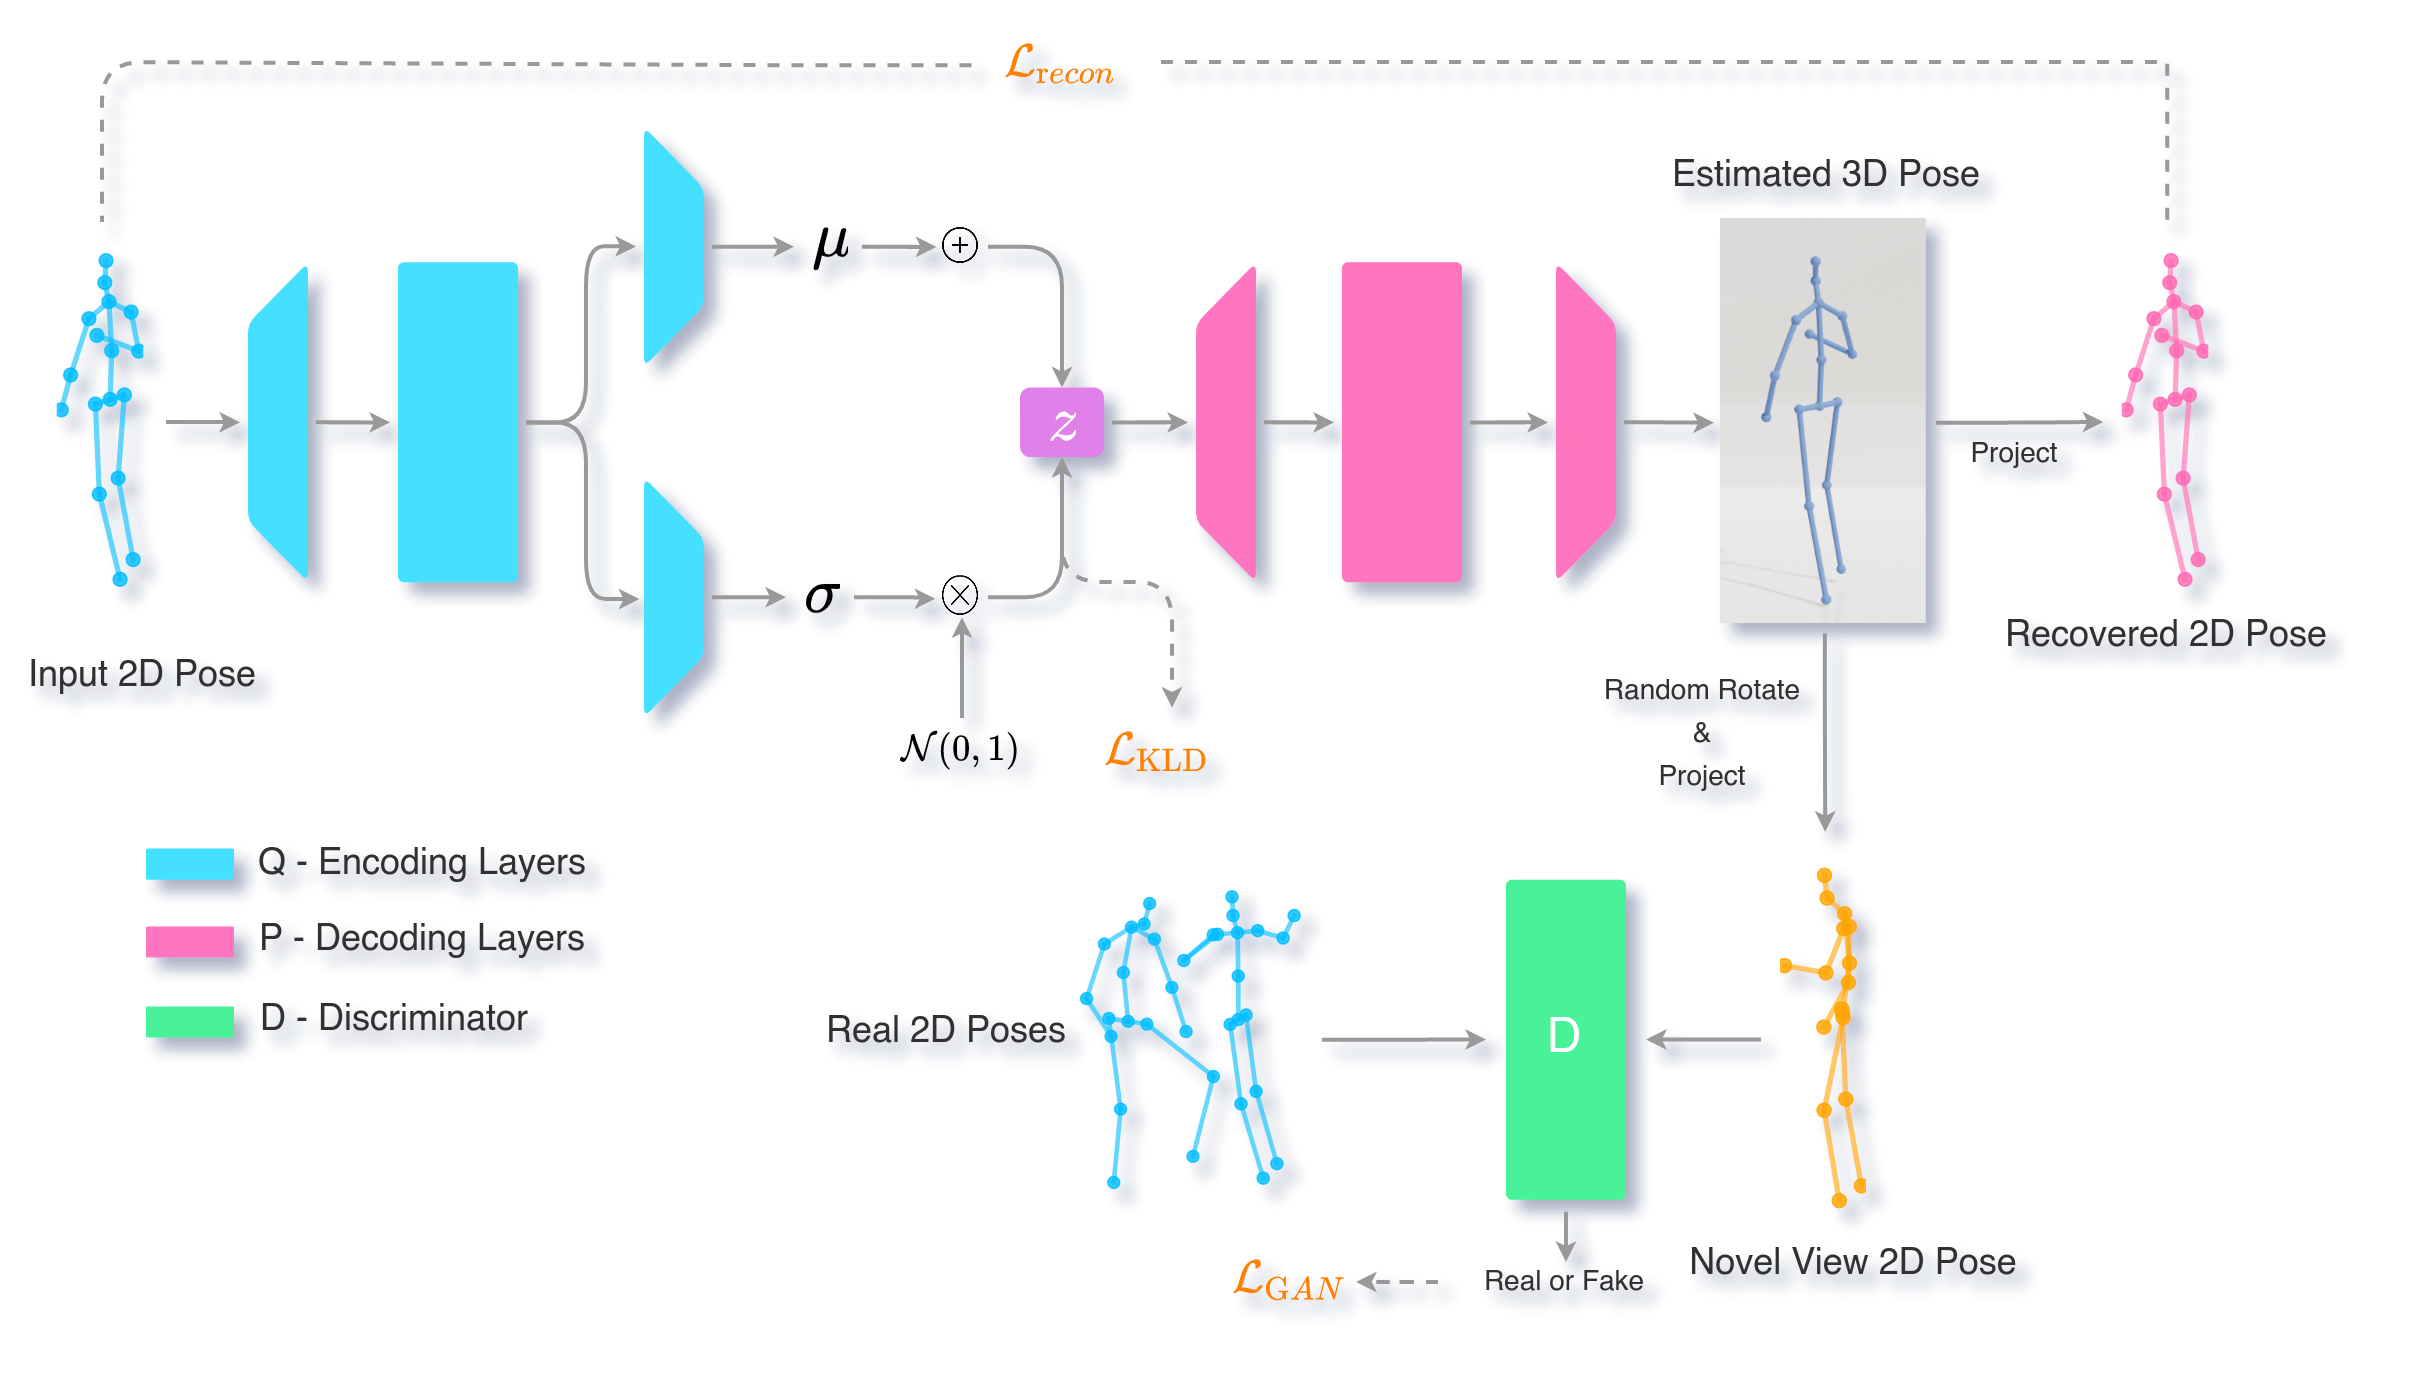
\includegraphics[width=\textwidth]{figures/arch/method_arch.png}
    \caption{Illustration of the neural architecture of the proposed method. The network components in blue, encode the 2D pose to a latent representation in terms of mean $\mu$ and standard deviation $\sigma$ of the distribution. While the components in pink, sample $z$ from this latent space and decode the corresponding 3D pose. The 3D pose is projected directly to 2D space for a constrained optimization using input 2D pose in the camera view and randomly rotated and projected for unconstrained optimization using the discriminator $D$ in a novel angle. The data that contributes to the loss function in orange, are mapped with a dotted line.
    }
\end{figure}

\section{Discriminator}
The discriminator takes the novel view 2D pose of the predicted 3D pose $\tilde{\textbf{y}}$ along with the real 2D poses \textbf{x} from the dataset as the input and classifies which 2D pose belongs to which cateogory, real or fake (generated novel view). The real and novel views need not correspond to the same pose, the goal of the discriminator is to learn the general ability to distinguish the 2D poses from the dataset (real) from the predicted poses (fake).

\begin{equation} \label{eqn:proj_rotated}
    \begin{gathered}[b]
        D_{\theta_d}(\tilde{\textbf{y}}, \textbf{x}) = P(0\leq class \leq 1)
    \end{gathered}
\end{equation}

Where $\theta_d$ refers to the learned parameters of the discriminator and $P(class)$ here denotes the probabilty of the pose's class, with 1 being real and 0 being fake. The discriminator mimicing the encoder and the decoder, upsamples the $2\!\cdot\!J$ dimensional novel 2D pose to $h$ dimensions of the main module. The main module just as other models is composed of $n$ residual blocks. It is important to note that $n$ need not be the same for all the 3 models. The learned features are downsampled to predict the probabilty of the pose being real or fake. The sigmoid activation function is used here as the required values are in the range [0, 1]. %TODO


\section{Training}

%TODO %%%%%%%%%%%%%%%%%%%%%%%%%%%%%%%%%%%%%%%%%%%%%%%%%%%%%%%%%%%%%%%%%%%%%%%%%
% Following the best practices from \cite{soumith2017wasserstein}, the decoder (and the encoder) which acts as the generator for the \ac{gan} is made to output 3D poses with values from [-1,1]. 
% %FIXME blunder in the implementation?
%%%%%%%%%%%%%%%%%%%%%%%%%%%%%%%%%%%%%%%%%%%%%%%%%%%%%%%%%%%%%%%%%%%%%%%%%
% initalization activation optimier
% at activation mention that the scaling of -1 again?
%TODO
% add parameters of the netowrks number of layers hidden dimension root at 0 16 joints prediciton 17 joints

The training scheme is similar to the standard \ac{vae} and \ac{vae}-\ac{gan} introduced in \ref{sec:Preliminary}. The discriminator is trained first for a few steps before training the \ac{vae}. First, the \ac{vae} takes the 2D pose as input and predicts the 3D pose. This predicted 3D pose is first reprojected to 2D to train the \ac{vae} and then randomly rotated and reprojected to a novel 2D view. This novel 2D is used as fake samples to train the discriminator. As \ac{vae} learns to improve the reprojected 2D pose, it will eventually be very close to the real samples. Using these as the fake examples will not be very useful as the decoder does the same job. Training the discriminator on a randomly rotated and reprojected 2D novel view would encourage the decoder to generate a pose that not only agrees with the input 2D pose but ensures that the other view of the 3D is also indistinguishable from the variations found in the data by fooling the discriminator. This two-view supervision leads to better 3D pose generations.


\subsection{More on Activation functions}
beta scheduling cycling and o to 1 annealing, weighting the loss components

%FIXME
\subsection{Loss Functions}
beta scheduling cycling and o to 1 annealing, weighting the loss components

\subsection{Optimizers Functions}
beta scheduling cycling and o to 1 annealing, weighting the loss components



\section{Evaluation Metrics} % FIXME
3D \ac{hpe} and Human3.6M in particular is mainly evaluated by \ac{mpjpe} metric. MPJPE as it abbreviates is the mean of the position estimate for all the joints of a pose. Where per-joint position estimate is nothing but the euclidian distance (usually measured in mm) between the predicted joint to its ground truth.


\begin{figure}[h]
    \centering
    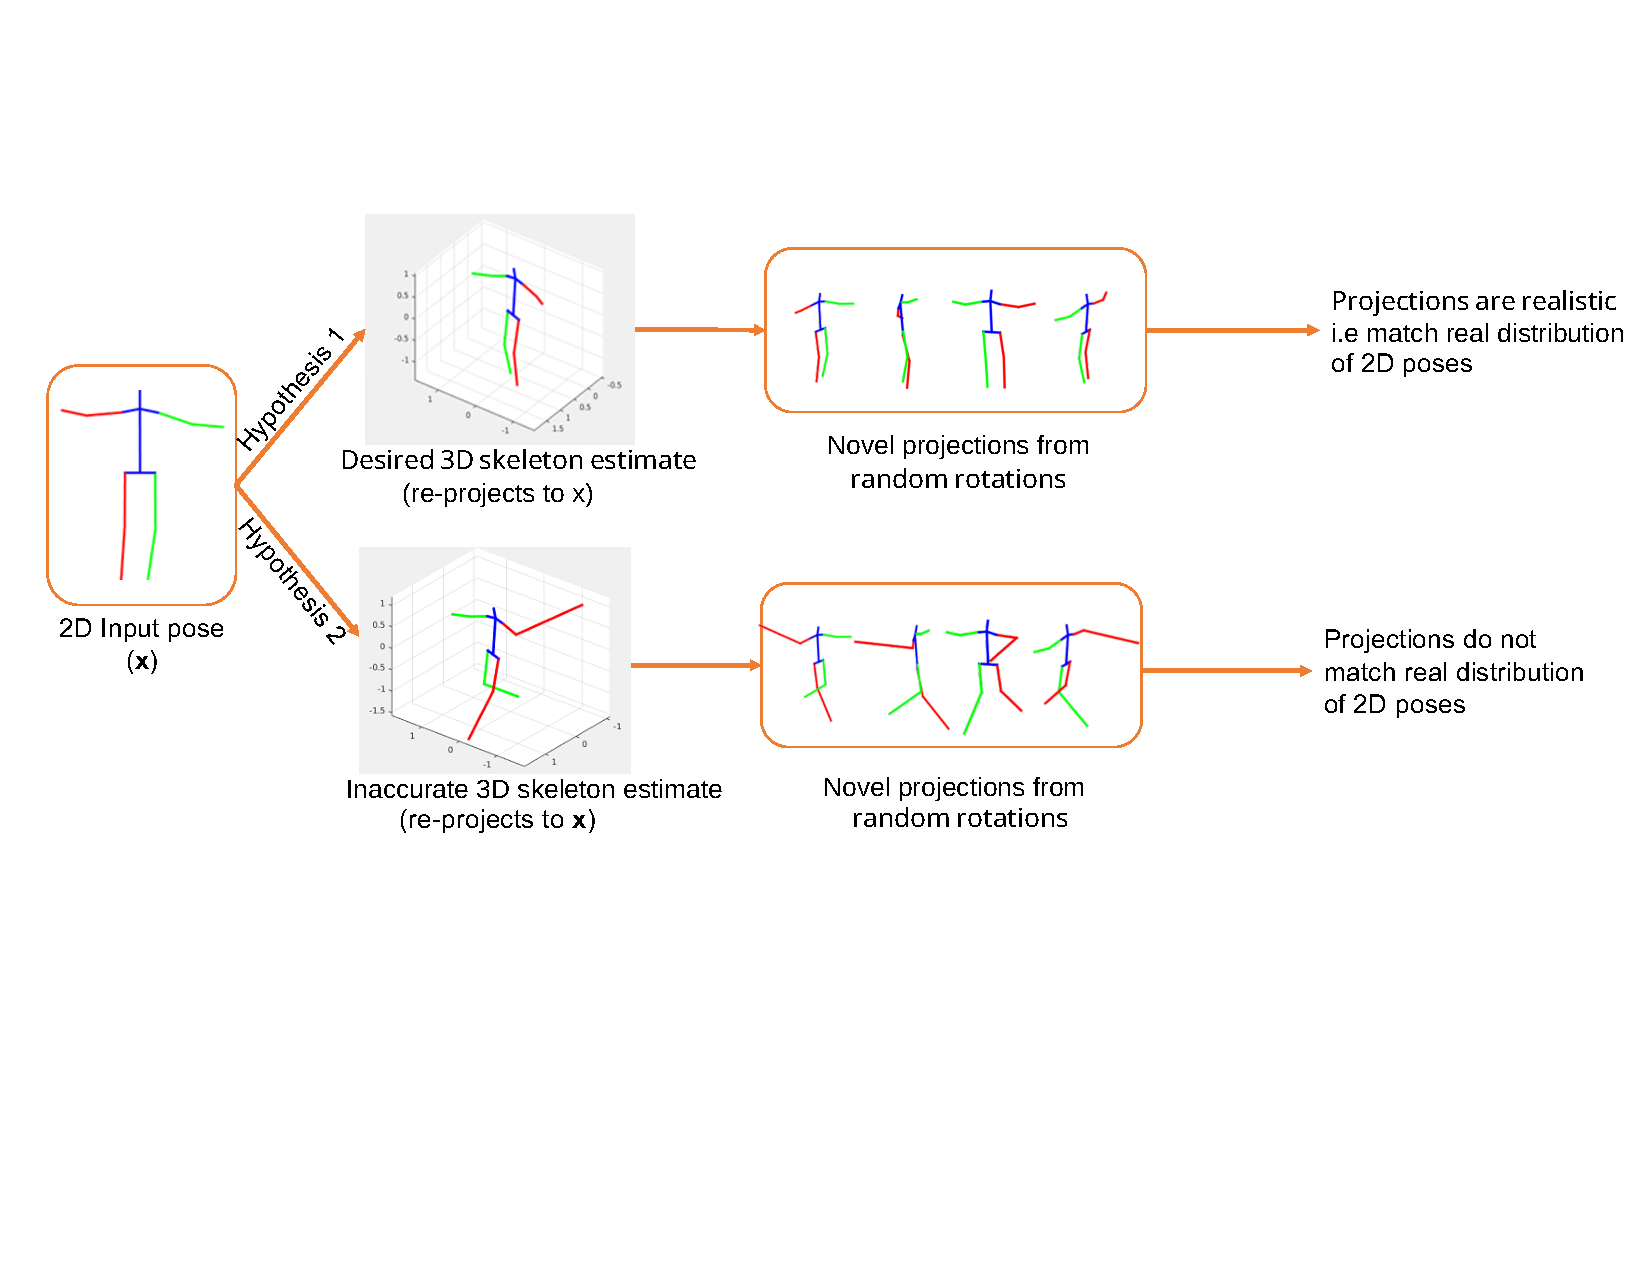
\includegraphics[width=\textwidth]{figures/h36_viz/novel_view_contraint.pdf}
    \caption{Illustration of the architecutre and loss flow in the proposed approach.}
    \label{fig:novel_view_constraint}
\end{figure}

% \section{more details the model prints?} % FIXME
%TODO add all models in apendix